% This file was created by matlab2tikz.
%
%The latest updates can be retrieved from
%  http://www.mathworks.com/matlabcentral/fileexchange/22022-matlab2tikz-matlab2tikz
%where you can also make suggestions and rate matlab2tikz.
%
\documentclass[tikz]{standalone}
\usepackage[tuenc]{fontspec}
\setmainfont{FreeSerif}
\usepackage{pgfplots}
\usepackage{grffile}
\pgfplotsset{compat=newest}
\usetikzlibrary{plotmarks}
\usetikzlibrary{arrows.meta}
\usepgfplotslibrary{patchplots}
\usepackage{amsmath}

\begin{document}
	\definecolor{mycolor1}{rgb}{0.00000,0.44700,0.74100}%
	\scriptsize
	\begin{tikzpicture}
	\scriptsize
	\useasboundingbox (-10mm,-10mm) rectangle (57.5mm,35mm);
%	\begin{axis}[%
%	width=52mm,
%	height=35mm,
%	at={(2mm,-2mm)},
%	scale only axis,
%	]
	
%	\end{axis}
	\put(57,-14) {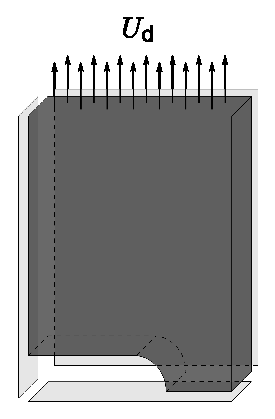
\includegraphics[angle=90,trim=0mm 0 0 5mm,clip,scale=.8]{./3d_plate_1_8.eps}}
	\put(-23,38) {$U_d$}
	\end{tikzpicture}%
	
\end{document}